
\documentclass[aspectratio=43]{beamer}
% Theme works only with a 4:3 aspect ratio
\usetheme{CSCS}

\usepackage{tikz}
\usepackage{pgfplots}
\usepackage{pgfplotstable}
\usetikzlibrary{pgfplots.groupplots,spy}
\usepackage{listings}
\usepackage{color}

% define footer text
\newcommand{\footlinetext}{Insert\_Footer}

% Select the image for the title page
\newcommand{\picturetitle}{cscs_images/image3.pdf}

% source code listing
\newcommand{\lst}[1]{\lstinline!#1!}
\newcommand{\lstfont}[1]{\color{#1}\scriptsize\ttfamily}

\lstset{
    language=[ANSI]C++,
    backgroundcolor=\color{white},
    basicstyle=\lstfont{blue},
    identifierstyle=\lstfont{blue},
    keywordstyle=\lstfont{blue},
    commentstyle=\lstfont{blue},
    breaklines=true
}

\definecolor{codenumber}{rgb}{0.5,0.5,0.5}
\definecolor{codekeyword}{rgb}{0.9,0.4,0.7}
\definecolor{codeCUDA}{rgb}{1.0,0.6,0.6}

\lstset{
    emph={
        cudaMemcpy,
        cudaMalloc,
        cudaFree,
        cudaMemcpyHostToDevice,
        cudaMemcpyDeviceToHost,
        cudaSuccess,
        cudaGetLastError,
        cudaGetErrorString,
        cudaErrorMemoryAllocation,
        cudaError_t
    },
    emphstyle={\bfseries\lstfont{codeCUDA}}
}

\lstdefinestyle{boxcuda}{
    language=[ANSI]C++,
    showstringspaces=false,
    backgroundcolor=\color{white!15!black},
    basicstyle=\lstfont{white},
    identifierstyle=\lstfont{white},
    keywordstyle=\lstfont{codekeyword},
    numberstyle=\lstfont{white},
    stringstyle=\lstfont{cyan},
    commentstyle=\lstfont{green!40!white},
    breaklines=true
}

% Please use the predifined colors:
% cscsred, cscsgrey, cscsgreen, cscsblue, cscsbrown, cscspurple, cscsyellow, cscsblack, cscswhite

\author{Ben Cumming, CSCS}
\title{Introduction to CUDA}
\subtitle{Summer School 2015}
\date{\today}

\begin{document}

% TITLE SLIDE
\cscstitle

% TABLE OF CONTENT SLIDE
% All options for table of contents:
% currentsection, currentsubsection, firstsection=xx, hideallsubsections, hideothersubsections, part=xx, pausesections, pausesubsections, sections=xx, sections={xx-yy}, sections={xx,yy}
%\cscstableofcontents[hideallsubsections]{Title}

% CHAPTER SLIDE
\cscschapter{Introduction}

%%%%
\begin{frame}[fragile]{Introduction to CUDA}
    \begin{info}{The plan}
        \begin{itemize}
            \item learn about the GPU programming model
            \item implement CUDA kernels for simple linear algebra
            \item learn how to orchestrate asynchronous computaion and communication on GPU
            \item a 2D stencil application
        \end{itemize}
    \end{info}

    \begin{info}{Prerequisites}
        \begin{itemize}
            \item I assume C++ knowledge
            \begin{itemize}
                \item I will be using C++11 (the bits that make C++ easier!)
                \item Fortran users consider working with a C++ user
            \end{itemize}
            \item No GPU or graphics experience required
        \end{itemize}
    \end{info}

\end{frame}

%%%%
\begin{frame}[fragile]{What is CUDA?}
    \begin{info}{A superset of C++}
        \begin{itemize}
            \item write CPU code using C++ (C++11 since CUDA 6.5)
            \item write kernels to run on GPU using new keywords
            \item provides special syntax for launching kernels on GPU
        \end{itemize}
    \end{info}

    \begin{info}{GPU specific}
        \begin{itemize}
            \item the CUDA extensions define the \emph{programming model}
            \item PRO : programming model is well suited to GPU
            \item CON : GPU-specific
        \end{itemize}
    \end{info}

    \begin{info}{Extras}
        \begin{itemize}
            \item provides library/API
            \item tools for profiling and debugging
        \end{itemize}
    \end{info}
\end{frame}

%%%%
\begin{frame}[fragile]{Device and Host Memory}
    \begin{center}
        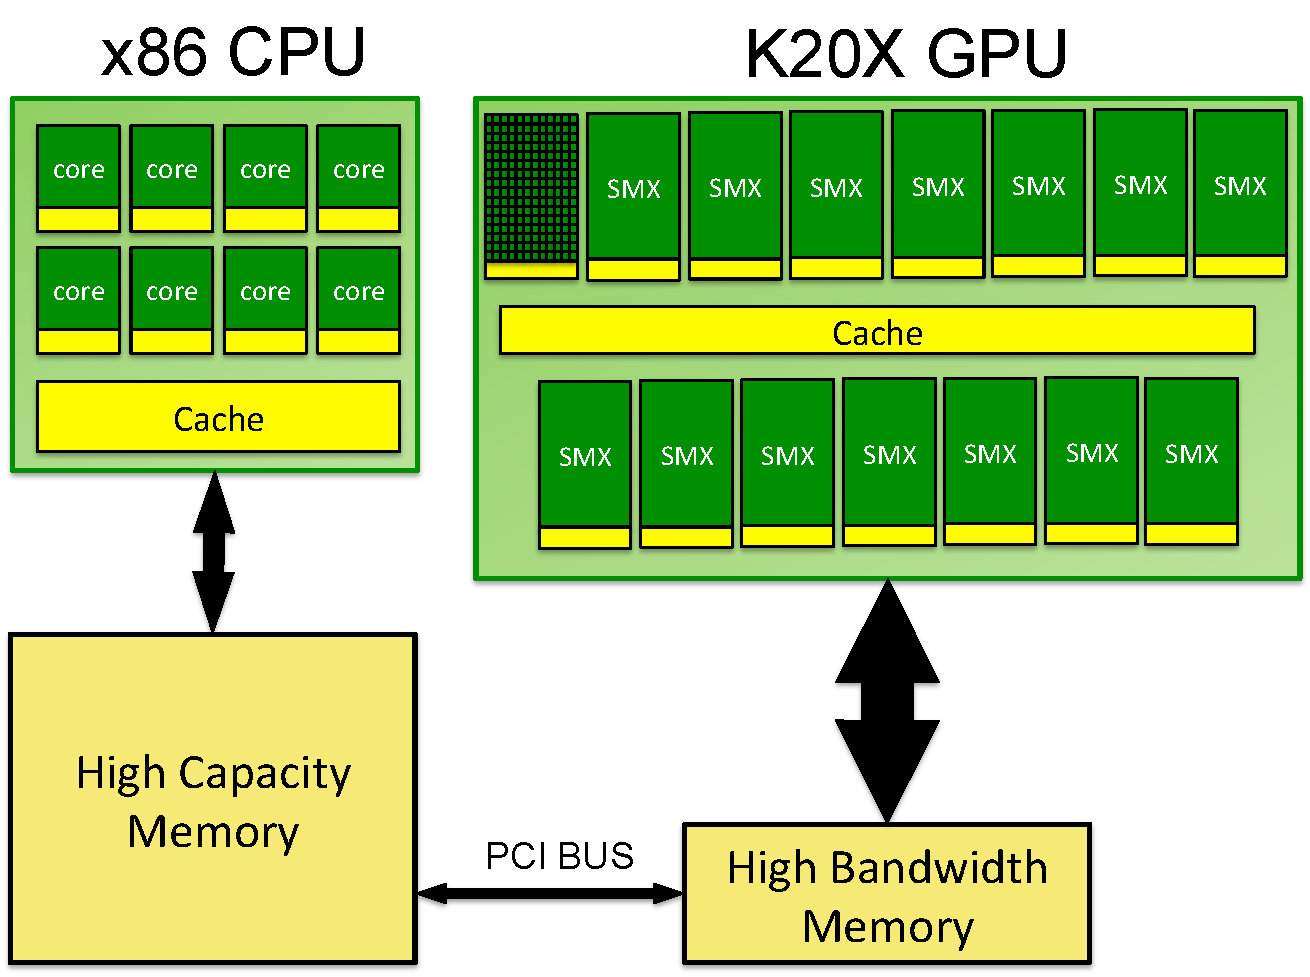
\includegraphics[width=0.9\textwidth]{./images/node.pdf}
    \end{center}
\end{frame}

%%%%
\begin{frame}[fragile]{Device and Host Memory}
    \begin{info}{host and device have separate memory spaces}
        \begin{itemize}
            \item data must be copied between host and device memory via PCI
            \item data must be in device memory for kernels to access
            \item ensure data is in the right memory space \emph{before} computation starts
                \begin{itemize}
                    \item PCIe2 = 6-12 GB/s
                    \item CPU socket = 35-50 GB/s
                    \item K20X  = 180 GB/s
                \end{itemize}
        \end{itemize}
    \end{info}

    \begin{info}{CUDA uses normal pointers to reference GPU memory}
        \begin{itemize}
            \item it isn't possible to tell whether a pointer points to device or host
            \item accessing a device pointer in host code is \emph{undefined behaviour}
        \end{itemize}
    \end{info}

\end{frame}

%%%%
\begin{frame}[fragile]{Allocating Memory}

    \begin{info}{allocating memory on device}
        \centering \lst{cudaMalloc(void **ptr, size_t size)}
    \begin{itemize}
        \item \lst{size} number of bytes to allocate
        \item \lst{ptr} points to allocated memory on exit
    \end{itemize}
    \end{info}

    \begin{info}{freeing memory on device}
        \centering \lst{cudaFree(void *ptr)}
    \end{info}

    \begin{code}{allocate 100 doubles on device}
%..................................
        \begin{lstlisting}[style=boxcuda]
double *v;
int size_in_bytes = 100*sizeof(double);
cudaMalloc(&v, size_in_bytes); // allocate memory
cudaFree(v);                   // free memory
\end{lstlisting}
%..................................
    \end{code}
\end{frame}

%%%%
\begin{frame}[fragile]{Copying data}

    \begin{info}{perform blocking copy (host waits for copy to finish)}
        \centering \lst{cudaMemcpy(void *dst, void *src, size_t size, cudaMemcpyKind kind)}
    \begin{itemize}
        \item \lst{dst} destination pointer
        \item \lst{src} source pointer
        \item \lst{size} number of \emph{bytes} to copy to \lst{dst}
        \item \lst{kind} enumerated type specifying \emph{direction} of copy:
            \lst{cudaMemcpyHostToDevice}, also \lst{DeviceToHost}, \lst{DeviceToDevice}
    \end{itemize}
    \end{info}

    \begin{code}{copy 100 doubles to device, then back to host}
%..................................
        \begin{lstlisting}[style=boxcuda]
double *v_d;
int size = sizeof(double)*100; // size in bytes
cudaMalloc(&v_d, size);
double *v_h = (double*)malloc(size);
cudaMemcpy(v_d, v_h, size, cudaMemcpyHostToDevice);
cudaMemcpy(v_h, v_d, size, cudaMemcpyDeviceToHost);
\end{lstlisting}
%..................................
    \end{code}
\end{frame}

%%%%
\begin{frame}[fragile]{Error handling}

    \begin{info}{}
        All API functions return error codes that indicate either:
        \begin{itemize}
            \item an error in the API call
            \item an error in an earlier asynchronous call
        \end{itemize}
        The return value is the enum type \lst{cudaError_t}
        \begin{itemize}
            \item e.g. \lst{cudaError_t status = cudaMalloc(&v, 100);}
            \begin{itemize}
                \item success : \lst{status==cudaSuccess}
                \item error   : \lst{status==cudaErrorMemoryAllocation}
            \end{itemize}
        \end{itemize}
    \end{info}

    \begin{info}{Handling errors}
        \lst{const char* cudaGetErrorString(status)}
        \begin{itemize}
            \item returns a string describing status
        \end{itemize}
        \lst{cudaError_t cudaGetLastError()}
        \begin{itemize}
            \item gets the \lst{cudaError_t} for the last error
        \end{itemize}
    \end{info}

\end{frame}

%%%%
\begin{frame}[fragile]{Error handling}

    \begin{code}{copy 100 doubles to device, with error checking}
%..................................
        \begin{lstlisting}[style=boxcuda]
double *v_d;
int size = sizeof(double)*100;
double *v_host = (double*)malloc(size);
cudaError_t status = cudaMalloc(&v_d, size);
if(status != cudaSuccess) {
  printf("cuda error : %s\n", cudaGetErrorString(status));
  exit(1);
}
status =
  cudaMemcpy(v_d, v_h, size, cudaMemcpyHostToDevice);
if(status != cudaSuccess) {
  printf("cuda error : %s\n", cudaGetErrorString(status));
  exit(1);
}
        \end{lstlisting}
%..................................
    \end{code}

    It is essential to test for errors
    \begin{itemize}
        \item but it gets tedious...
    \end{itemize}
\end{frame}

%%%%
\begin{frame}[fragile]{Exercise: API Basics}

    Open \lst{cuda/exercises/util.h}
    \begin{enumerate}
        \item what does \lst{cude_check_error()} do?

        \item Write a template wrapper around cudaMalloc to simplify allocating memory
        \begin{itemize}
            \item use the example for \lst{malloc_host} that is already implemented
            \item remember to check for errors API errors.
            \item what are the benefits over using \lst{cudaMalloc} directly?
            \item do we need to write a similar function for \lst{cudaFree}?
        \end{itemize}

        \item Write a wrapper around \lst{cudaMemcpy} for copying data from host to device
        \begin{itemize}
            \item use the example for the reverse operation \lst{copy_device_to_host_sync}
        \end{itemize}

        \item Compile the test and run
        \begin{itemize}
            \item it will pass with no errors on success
        \end{itemize}
    \end{enumerate}

\end{frame}

% THANK YOU SLIDE
\cscsthankyou{Thank you for your attention.}

\end{document}
